  \documentclass[a4paper,10pt]{article}

  \usepackage{fullpage}
  \usepackage{xcolor}
  \usepackage{graphicx}
  \usepackage{amsmath}
  \usepackage{amssymb}
  \usepackage{hyperref}
  \usepackage{url}
  \usepackage{float}
  \hypersetup{
      colorlinks=true,       % false: boxed links; true: colored links
      linkcolor=blue,          % color of internal links
      citecolor=green,        % color of links to bibliography
      filecolor=magenta,      % color of file links
      urlcolor=cyan           % color of external links
  }

  % Title Page
  \title{BTK developers documentation}
  \author{Fbrain ERC project: Computational Anatomy of Fetal Brain}


  \begin{document}
  \maketitle
  \tableofcontents
  %\begin{abstract}
  %\end{abstract}

  \section{Introduction}

  BTK stands for Baby Brain Toolkit. This toolkit is developed in the context of
  the Fbrain ERC project: ``Computational Anatomy of Fetal
  Brain''\footnote{http://lsiit-miv.u-strasbg.fr/miv/index.php?contenu=erc}. 
  Studies about brain maturation aim at providing a better understanding of brain
  development and links between brain changes and cognitive development. Such
  studies are of great interest for diagnosis help and clinical course of
  development and treatment of illnesses. Several teams have begun to make 3D maps
  of developing brain structures from children to young adults. However, working
  out the development of fetal and neonatal brain remains an open issue. This
  project aims at jumping over several theoretical and practical barriers and at
  going beyond the formal description of the brain maturation thanks to the
  development of a realistic numerical model of brain aging.

  \subsection{Copyright}
  This software is governed by the CeCILL-B license under French law and
  abiding by the rules of distribution of free software.  You can  use, 
  modify and/ or redistribute the software under the terms of the CeCILL-B
  license as circulated by CEA, CNRS and INRIA at the following URL: \url{http://www.cecill.info}. 

  As a counterpart to the access to the source code and rights to copy,
  modify and redistribute granted by the license, users are provided only
  with a limited warranty  and the software's author,  the holder of the
  economic rights,  and the successive licensors  have only  limited
  liability. 

  In this respect, the user's attention is drawn to the risks associated
  with loading,  using,  modifying and/or developing or reproducing the
  software by the user in light of its specific status of free software,
  that may mean  that it is complicated to manipulate,  and  that  also
  therefore means  that it is reserved for developers  and  experienced
  professionals having in-depth computer knowledge. Users are therefore
  encouraged to load and test the software's suitability as regards their
  requirements in conditions enabling the security of their systems and/or 
  data to be ensured and,  more generally, to use and operate it in the 
  same conditions as regards security. 

  Any researcher reporting results using BTK should acknowledge this software by citing the following article:
  \begin{enumerate}
 \item F. Rousseau, E. Oubel, J. Pontabry, M. Schweitzer, C. Studholme, M. Koob, J.-L. Dietemann: BTK: An Open-Source Toolkit for Fetal Brain MR Image Processing. Computer Methods and Programs in Biomedicine, pp. 65--73, Vol. 109, Num. 1, January 2013, also available on \href{http://hal.archives-ouvertes.fr/index.php?halsid=d0mrvug09qhhou49vgaqc6ogd3&view_this_doc=hal-00671183&version=1}{HAL}.
  \end{enumerate}

  \subsection{Installation}

  \subsubsection{Dependencies}

  Baby Brain Toolkit (BTK) is written in C++ and needs the following packages\footnote{BTK has been tested under Debian 5.0 and MacOSX 10.6.8}:
  \begin{itemize}
  \item \href{http://www.cmake.org}{CMake}, \href{http://tclap.sourceforge.net}{Tclap}, \href{http://openmp.org}{OpenMP}, \href{http://www.vtk.org}{VTK}, ANN (www.cs.umd.edu/\string~mount/ANN) and Doxygen. These
  libraries can be installed using the following command line: 
  \begin{itemize}
  \item for debian-based distributions: \texttt{apt-get install cmake
  cmake-curses-gui libtclap-dev libgomp1 libann-dev doxygen}
  \item for MacOSX using macports\footnote{When configuring in cmake, please use /opt/local/include for TCLAP\_DIRECTORY}: \texttt{port install cmake tclap libANN doxygen}
  \end{itemize}
  \item Install Git: this library can be installed using the following command line : 
  \begin{itemize}
  \item for debian-based distribution: \texttt{apt-get install git-core}
  \item for MacOSX using macports: \texttt{port install git-core}
  \end{itemize}
  \item \href{http://www.itk.org/ITK/resources/software.html}{Insight Toolkit (ITK) version 4.3.1}
  \begin{itemize}
  \item Download the tar.gz archive of ITK v4.3.1
  \item Extract the archive 
  \item Then open a terminal and type :
  \end{itemize}
  \begin{verbatim}
  mkdir ITK-build
  cd ITK-build
  ccmake ../(your-ITK-Source-folder)/
  \end{verbatim}
  This will bring up the CMake configuration screen. Press \texttt{[c]} for
  configure and then use \texttt{[t]} to toggle the advanced mode. Make the
  following changes:
  \begin{verbatim}
  BUILD_TESTING = OFF
  ITK_USE_REVIEW = ON
  ITK_BUILD_ALL_MODULES = ON
  ITKV3_COMPATIBILITY = ON
  BUILD_DOCUMENTATION = OFF
  CMAKE_BUILD_TYPE = Release
  \end{verbatim}
  Or for debugging and development purpose :
  \begin{verbatim}
  CMAKE_BUILD_TYPE = Debug

  \end{verbatim}
  Then press \texttt{[c]} to configure and \texttt{[g]} to generate the make file.
  Finally, go to the build folder of ITK (ITK-build) and type \texttt{make} at the prompt to obtain the final build of ITK.
   \item \href{http://www.vtk.org/VTK/resources/software.html#previous}{Visualization ToolKit (VTK) version 5.10.1 }
 \begin{itemize}
 \item Download the tar.gz archive of VTK v5.10.1
 \item Extract the archive 
 \item Then open a terminal and type :
 \end{itemize}
  \begin{verbatim}
  mkdir VTK-build
  cd VTK-build
  ccmake ../(your-VTK-Source-folder)/
  \end{verbatim}
  This will bring up the CMake configuration screen. Press \texttt{[c]} for
  configure and then use \texttt{[t]} to toggle the advanced mode. Make the
  following changes:
  \begin{verbatim}
  BUILD_TESTING = OFF
  BUILD_EXAMPLE = OFF
  CMAKE_BUILD_TYPE = Release
  \end{verbatim}
  Or for debugging and developement purpose :
  \begin{verbatim}
  CMAKE_BUILD_TYPE = Debug

\end{verbatim}

  \end{itemize}

  \subsubsection{Download the BTK sources}

  \begin{itemize}
  \item Get the BTK sources:
    \begin{itemize}
    \item For the Latest stable version :
    \begin{verbatim}
    git clone https://github.com/rousseau/fbrain.git
    git checkout Btk_1.0 
    \end{verbatim}
    \item For the current development version :
    \begin{verbatim}
    git clone https://github.com/rousseau/fbrain.git
    \end{verbatim}  
    \end{itemize}
  \item Then for compiling:
  \begin{verbatim}
  mkdir fbrain-build
  cd fbrain-build
  ccmake ../fbrain
  \end{verbatim}
  Make the following changes on the CMake configuration screen :
  \begin{verbatim}
  ITK_DIR = (YOUR-ITK-BUILD-FOLDER)
  VTK_DIR = (YOUR-VTK-BUILD-FOLDER)
  CMAKE_BUILD_TYPE = Release
  \end{verbatim}
  Or for debugging and developement purpose :
  \begin{verbatim}
  CMAKE_BUILD_TYPE = Debug
  \end{verbatim}
  then :
  \begin{verbatim}
  make
  \end{verbatim}

  \end{itemize}

  Most of the programs of the BTK suite use the OpenMP library for multi-threading
  purpose. The number of cores used can be tuned using the following command line
  (in this example, 4 cores will be used): \texttt{export OMP\_NUM\_THREADS=4}


      \section{Development}
    This part contain all informations needed to develop new programs in BTK.

    \subsection{BTK tree}
    BTK is build using a tree.
    The source code is contained into the \textit{Code} folder.
    Programs are respectively into \textit{Applications} and \textit{Utilities}.
    \textit{Documentation} and \textit{Medias} contain the documentation and some pictures for the \href{http://rousseau.github.com/fbrain/}{Website of the project}

    \begin{figure}[H]
     \centering
      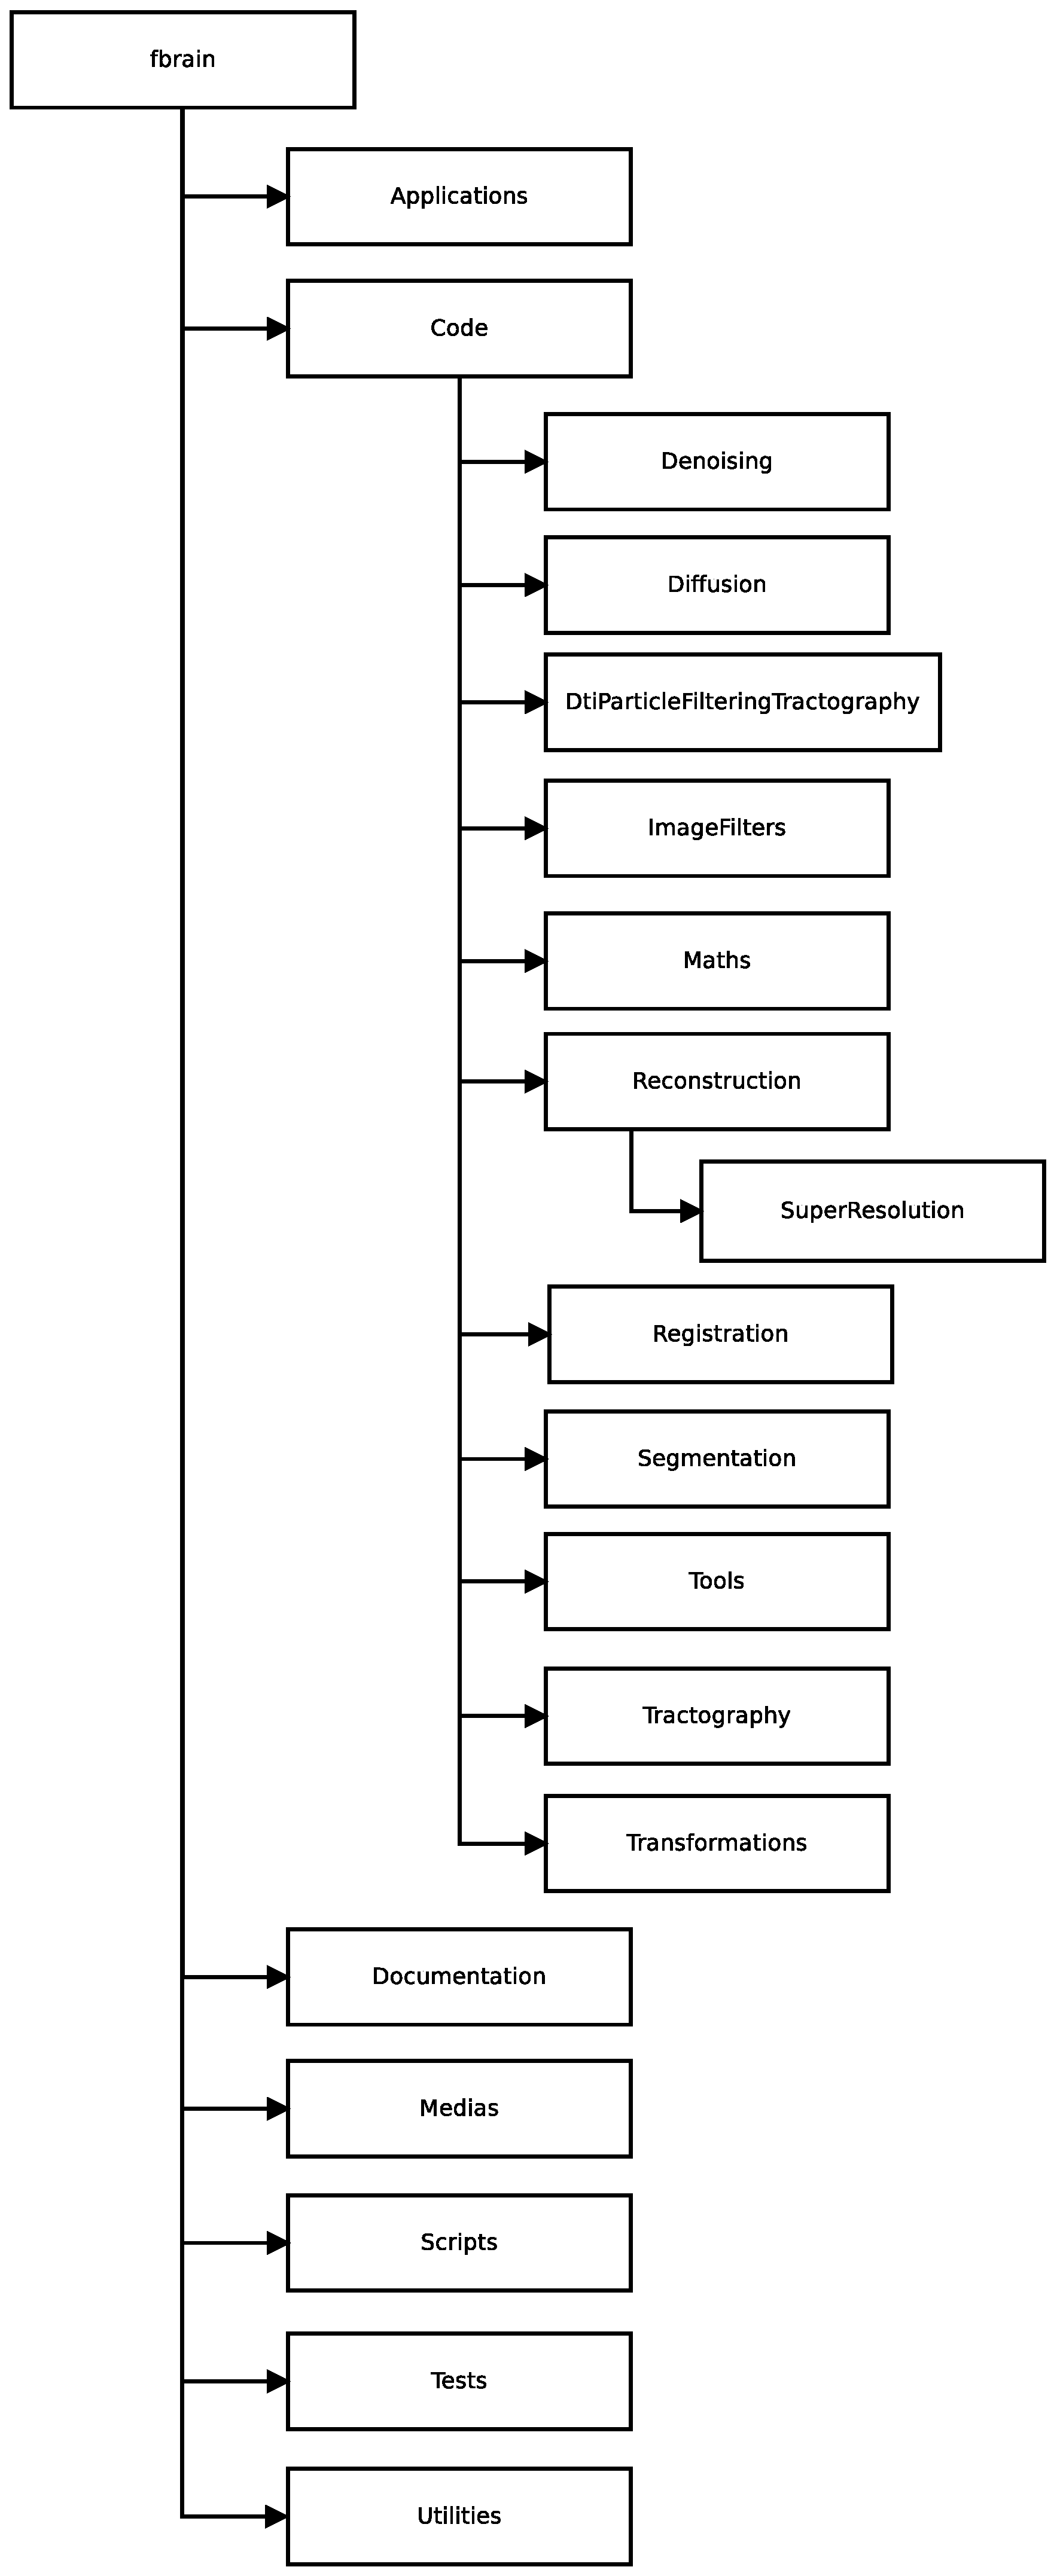
\includegraphics[height=0.5\textwidth]{Btk_tree.eps}
      \caption{Tree of BTK.}
    \end{figure}

    \subsection{Standards}
    Since BTK is written in C++, we use standards, most of time the standards come from ITK library.\\

    \begin{itemize}
    \item Name of Class :\\
      Capital letter at the begining and then CamelCase\footnote{ http://en.wikipedia.org/wiki/CamelCase} :
      \begin{verbatim}
      class MyClass
      class MySuperClass
      \end{verbatim}

    \item Variable member of a Class :\\
      m\_ at the beginin, then a Capital letter and the next in CamelCase :
      \begin{verbatim}
      int m_MyVariable
      \end{verbatim}

    \item Fonction member of a Class :\\
      Capital letter at the begining and then CamelCase :
      \begin{verbatim}
      void MyFonction()
      void MySuperFonction()
      \end{verbatim}

    \item Conditions, loops, instructions... :\\
      Brackets at the line and aligned
      \begin{verbatim}
      for(int i = 0; i < 3; i++)
      {
        //some stuff
      }
      void MySuperFonction()
      {
      
      }
      \end{verbatim}

    \item Constants, enum... :\\
      All letter of the word in capital letter, if composed word separated it by a \_
      \begin{verbatim}
       enum AXES
       {
           AXIAL =0,
           SAGITTAL,
           CORONAL
       } ;

       MY_CONSTANT TRUE = true;
      \end{verbatim}

    \end{itemize}

    Don't forget the C++ standards and be the more logical you can when programming !

    \subsection{Helper classes}
    In BTK we have some helper classes. As their names suggests,those classes are created for helping the programmer for usual fonctions.
    \subsubsection{btkImageHelper}
    \begin{itemize}
    \item File : Code/Tools/btkImageHelper.(h/txx)
    \item Using : Class of static fonctions for create, read, write a image or a vector of images
    \item example :
      \begin{verbatim}
      #include "btkImageHelper.h"
                 
      typedef itk::Image<short, 3> itkImage;
      
      std::string inputFileName = "inputImage.nii.gz";      
      itkImage::Pointer image = btk::ImageHelper<itkImage>::ReadImage(inputFileName);
      
      std::string outputFileName = "outputImage.nii.gz";
      btk::ImageHelper<itkImage>::WriteImage(image, outputFileName);

      \end{verbatim}
    \end{itemize}

    \subsubsection{btkFileHelper}
    \begin{itemize}
    \item File : Code/Tools/btkFileHelper.(h/txx)
    \item Using : Class of static fonctions for check if a file exist or a vector of files
    \item example :
      \begin{verbatim}
      #include "btkFileHelper.h"

      std::string filename("MyName");
      bool fileExist = btk::FileHelper::FileExist(filename);
      \end{verbatim}

    \end{itemize}

    \subsubsection{btkIOTransformHelper}
    \begin{itemize}
    \item File : Code/Tools/btkIOTransformHelper.(h/txx)
    \item Using : Class of static fonctions for reading and writing transforms, this class is currently under developpment !
    \item example :
      \begin{verbatim}
      #include "btkIOTransformHelper.h"

     typedef itk::AffineTransform<double,3> Transform;
     Transform::Pointer transform = Transform::New();
     transform->SetIdentity();

     std string filename("MyName");

     btk::IOTransformHelper<Transform>::WriteTransform(transform,filename);
      
      \end{verbatim}

    \end{itemize}

    \subsubsection{btkMacro}
    \begin{itemize}
    \item File : Code/Tools/btkMacro.h
    \item Using : File with some macro for Set/Get variable into classes
    \item example :
      \begin{verbatim}
      #include "btkMacro.h"

      namespace btk
      {
      class MyClass:
      {
      public:
      // the macro remove the m_ at the begining of the variable
      btkSetMacro(MyVariable,int); 
      btkGetMacro(MyVariable,int);

      private:
      int m_MyVariable;

      };
      }

      \end{verbatim}


    \end{itemize}
  \subsection{Doxygen}
  In order to generate a clear documentation, we using doxygen, so for your classes you should add comments in doxygen spirit.
  Here is a dummy example :
  \begin{verbatim}
#ifndef __MYCLASS_H__
#define __MYCLASS_H__

/*!
 * \file MyClass.h
 * \brief MyClass class
 * \author Luke Skywalker
 * \version 0.1
 */


/*! \namespace btk
 * 
 * namespace to contain all btk composants
 */
namespace btk
{
  /*! \class MyClass
   * \brief class for doing some magical things
   *
   *  Description of the class
   */
  class MyClass
  {
                                               
  public:
    /*!
     *  \brief Constructor
     *
     *  Constructor of the MyClass class
     *
     *  
     */
    MyClass();

    /*!
     *  \brief Destructor
     *
     *  Destructor of the MyClass class
     */
    virtual ~MyClass();

  protected :
  /*!
   *  \brief DoSomething
   *
   *  This method do something
   * \param value : integer value for doing something
   */
  void DoSomething(int value);

  /*!
   *  \brief DoAnotherThing
   *
   *  This method do something
   * \param value : integer value for doing something
   * \return bool : return true if value > 5 else return false
   */
  bool DoAnotherThing(int value);

  private:
  
  int m_MyVariable;/*!< My Variable for doing things*/

  };
};


  \end{verbatim}

     

\subsection{Create a new program}
First of all, you should know that in Btk we have two kind of programs, the first is the \textit{Application} programs which contain the importants programs (for the research project)
and the second is \textit{Utilities} which contain tools and Helpful programs.\\
Creating a new executable program is separated into two steps.
In first you should create a file.cxx which will contained your main
Next you should add your program (and the nessesary includes ) in the corresponding CMake file.\\

\subsubsection{Create a main}
You must create a new file with name of your choice for example btkImageReconstruction.cxx .
If your program take arguments (ie: input/output), you should use TCLAP\footnote{See the documentation http://tclap.sourceforge.net/html/index.html } library.
\subsubsection{Add the programm into CMake}
When your main program is written, you must add it into the CMake file.
Note that there are two CMake files , one for the \textit{Application} and the other for \textit{Utilities}.

Here is a example :
\begin{verbatim}
 ADD_EXECUTABLE(btkTensorStreamlineTractography
        btkTensorStreamlineTractography.cxx
        ${fbrain_SOURCE_DIR}/Code/Tractography/btkCartesianCoordinates.cxx
        ${fbrain_SOURCE_DIR}/Code/Tractography/btkSphericalCoordinates.cxx
        ${fbrain_SOURCE_DIR}/Code/Tractography/btkVector.cxx
        ${fbrain_SOURCE_DIR}/Code/Tractography/btkDirection.cxx
        ${fbrain_SOURCE_DIR}/Code/Tractography/btkPoint.cxx
        ${fbrain_SOURCE_DIR}/Code/DtiParticleFilteringTractography/btkDTFPSignalExtractor.cxx
        ${fbrain_SOURCE_DIR}/Code/DtiParticleFilteringTractography/btkDTFPSignal.cxx
        ${fbrain_SOURCE_DIR}/Code/Tractography/btkSphericalHarmonics.cxx
)

TARGET_LINK_LIBRARIES(btkTensorStreamlineTractography ${ITK_LIBRARIES} vtkHybrid)

INSTALL(TARGETS btkTensorStreamlineTractography
        DESTINATION bin)
\end{verbatim}


..TODO..



  \section*{Acknowledgment}
  \small{The research leading to these results has received funding from the
  European Research Council under the European Community’s Seventh Framework
  Programme (FP7/2007-2013 Grant Agreement no. 207667).}


  \end{document}
